\label{s:dataset_drive}
The publicly available DRIVE dataset~\cite{Staal_etal_TMI04} contains 40 full colour, JPEG compressed retinogram images (\fref{f:retinography}a) that originate from a diabetic neuropathy screening program in The Netherlands, where subjects were aged 25-90. The images were acquired using a Canon CR5 non-mydriatic 3CCD camera with a 45 degree field of view (FOV) and 8 bits per colour plane, and are $768 \by 584$ pixels in size. The field of view is defined by a mask, provided with every image, that results in a cropped image $565 \by 584$ pixels in size.

Forty images from a total of 400 were selected for the dataset, seven of which exhibit signs of mild early diabetic retinopathy. These 40 are split into 20 training and 20 test images. Every image comes with at least one mask (test images have two), hand-labelled by human observers, that define ground truth vessel segmentations (\fref{f:fig_drive_examples}).

\begin{figure}
\centering
\begin{tabular}{c c}
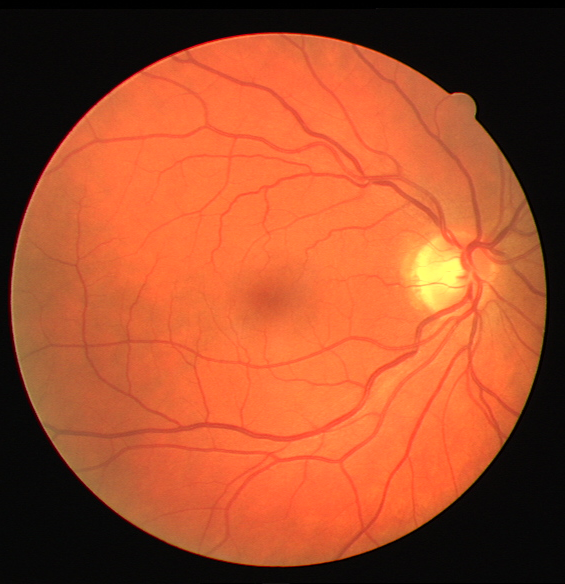
\includegraphics[width=\halfcol]{\figpath/retina/02_test} &
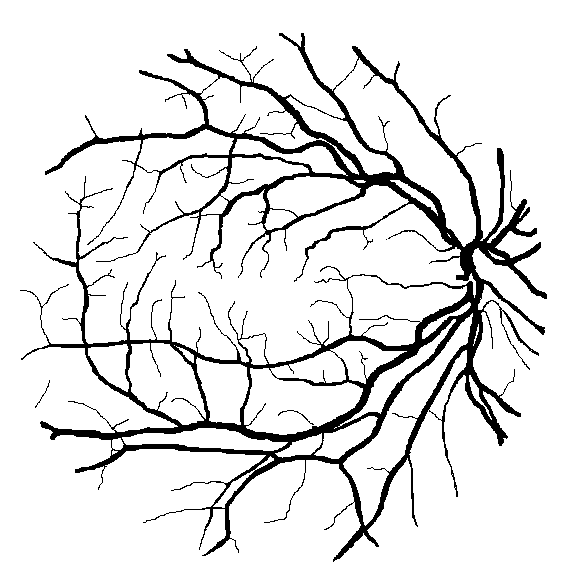
\includegraphics[width=\halfcol]{\figpath/retina/02_manual1} \\
(a) & (b) \\
\end{tabular}
%
\caption{(a) Typical image from DRIVE dataset; (b) corresponding ground truth segmentation.}
\label{f:drive_examples}
\end{figure}


